\documentclass[11pt]{article}
\usepackage[margin=1in]{geometry}
\usepackage{booktabs}
\usepackage{float}
\usepackage{graphicx}
\graphicspath{{../figures/}{figures/}}
\usepackage{amsmath, amssymb}
\usepackage{microtype}
\usepackage[breaklinks=true,colorlinks=true,linkcolor=black,citecolor=black,urlcolor=blue]{hyperref}

\title{Reproduction of \textit{IterAlign: Iterative Constitutional Alignment of Large Language Models}}
\author{NLP Assignment 2 Reproduction Report}
\date{\today}

\begin{document}
\maketitle

\begin{abstract}
This report reproduces the main claim of \textit{IterAlign}~\cite{chen2024iteralign}, an iterative constitutional alignment method that derives constitutions from a model's own harmful outputs and uses them to build supervised fine-tuning data without human preference labels. The original paper trains Llama-2-7B with full-parameter FSDP across eight A100 GPUs and serves it with vLLM, which places the full setup well beyond a typical course-project environment. The cloned repository used here contains both the original \texttt{constitution\_induced\_inference\_iterated\_llama2.py} script and a later \texttt{iteralign\_smollm.py} adaptation that replaces vLLM with Hugging Face Transformers, replaces GPT-3.5 with Gemini 3.1 Flash Lite, and targets a compact SmolLM-style setup on a single GPU. The repository also includes the processed prompt pickles and \texttt{bad\_cases\_all\_sorted.pkl}, so the few-shot seed file is available directly in the fork. The final artifact used for submission is a Gemini-judge comparison across four smoll-llm-135M training setups. In that comparison, every aligned variant outperforms the vanilla baseline: 0.42 for hh-rlhf, 0.45 for HarmfulQA, and 0.46 for DangerousQA versus 0.23 for vanilla. Section~\ref{sec:results} reports those results, and the rest of the report explains how to interpret them.
\end{abstract}

\section{Introduction}
\label{sec:intro}

Aligning large language models (LLMs) for harmlessness has usually depended either on expensive human preference data, as in InstructGPT/RLHF~\cite{ouyang2022instructgpt}, or on hand-written constitutions used as AI feedback, as in Anthropic's Constitutional AI (CAI)~\cite{bai2022cai}. Both approaches assume access to substantial human effort: either annotation at scale or carefully written normative principles. \textit{IterAlign}~\cite{chen2024iteralign} takes a different route. It first \emph{elicits} harmful behavior with red-team prompts~\cite{ganguli2022redteam}, then asks a stronger oracle model to \emph{induce} a short constitution from the bad outputs, and finally has the model \emph{regenerate} answers under that induced constitution. Those revised answers become a supervised fine-tuning (SFT) set. Repeating the loop yields progressively safer checkpoints along with a growing list of constitutions that reflect the model's failure modes.

This report is grounded in the repository snapshot cloned for submission. That matters because the fork already differs from the paper release: it contains the original Llama-2/vLLM script, a newer small-model adaptation script, and bundled processed data files that change what can be reproduced directly from the repo. Section~\ref{sec:paper} reviews the method and places it against RLHF and CAI. Section~\ref{sec:impl} explains how the cloned repository is organized and where it departs from the paper's original setup. Section~\ref{sec:setup} specifies the hardware, datasets, hyperparameters, and evaluation protocol. Section~\ref{sec:results} presents the final reproduced results, and Section~\ref{sec:repro} discusses where agreement or drift relative to the original paper is most likely.

\section{Paper Overview}
\label{sec:paper}

\subsection{Background and motivation}
The dominant alignment recipe for chat assistants is Reinforcement Learning from Human Feedback (RLHF)~\cite{ouyang2022instructgpt}. RLHF requires (i) a base SFT model, (ii) a sizeable preference dataset over response pairs, and (iii) a learned reward model trained to predict that preference. This pipeline produces strong assistants but is expensive: collecting preference pairs at scale is the dominant cost. Constitutional AI~\cite{bai2022cai} reduces the human-label cost by replacing human raters with an LLM judge that scores responses against a hand-authored constitution; this still requires careful prompt engineering to write the constitution itself.

\textit{IterAlign}~\cite{chen2024iteralign} removes both of those requirements. It does not need preference labels, and it does not start from a hand-written constitution. Instead, it extracts constitutions from cases where the current model already fails. The resulting rules are therefore tied to the model's observed weaknesses on the chosen red-team distribution. The revised SFT data also stays close to the task distribution, since it comes from re-prompting the same model under the newly induced constitution rather than importing answers written elsewhere.

\subsection{The IterAlign algorithm}
Let $M_0$ denote the base model, $\mathcal{D}_{\text{red}}$ a pool of red-team prompts (we use the Anthropic hh-rlhf-derived pool shipped in the repo, i.e.\ \texttt{initial\_red\_teaming\_data\_all.pkl}), $\Phi$ an oracle LLM (GPT-3.5 in the paper, Gemini 3.1 Flash Lite here), and $K$ the number of iterative rounds. Algorithm~\ref{alg:iteralign} summarises one round.

\begin{figure}[h]
\centering
\fbox{\parbox{0.95\linewidth}{
\textbf{Algorithm 1 (IterAlign --- one iterative round; mirrors the paper's Algorithm~1).}\\[2pt]
\textbf{Inputs:} current model $M_t$, prompt batch $\mathcal{P}_t \subset \mathcal{D}_{\text{red}}$, oracle $\Phi$, few-shot bad-cases $\mathcal{B}$, cumulative SFT pool $\mathcal{S}_t$, base model $M_0$.\\[3pt]
\begin{enumerate}
  \item $\mathcal{R}_t \gets \{ M_t(p) \mid p \in \mathcal{P}_t \}$ \hfill\textit{// red-team responses}
  \item $\mathcal{N}_t \gets \{ (p, r) \in \mathcal{P}_t \times \mathcal{R}_t : \Phi_{\text{cls}}(r \mid \mathcal{B}) = \text{Negative} \}$
  \item \textbf{if} $\mathcal{N}_t = \emptyset$ \textbf{then return} $(M_t, \mathcal{S}_t)$
  \item $c_t \gets \Phi_{\text{induce}}\!\left(\bigoplus_{(p,r) \in \mathcal{N}_t} r\right)$ \hfill\textit{// constitution from merged negatives}
  \item $\widetilde{\mathcal{R}}_t \gets \{ M_t(\text{Inject}(p, c_t)) \mid (p, \cdot) \in \mathcal{N}_t \}$
  \item $\mathcal{S}_{t+1} \gets \mathcal{S}_t \cup \{ (p, \tilde r) \mid (p, \cdot) \in \mathcal{N}_t,\ \tilde r \in \widetilde{\mathcal{R}}_t \}$
  \item $M_{t+1} \gets \text{SFT}(M_0, \mathcal{S}_{t+1})$ \hfill\textit{// train from base on cumulative pool}
  \item \textbf{return} $(M_{t+1}, c_t, \mathcal{S}_{t+1})$
\end{enumerate}
}}
\label{alg:iteralign}
\end{figure}

Three design choices matter here. First, each SFT step trains from the original base model on the \emph{cumulative} revised-pair pool $\mathcal{S}_{t+1}$ rather than warm-starting from $M_t$. That matches the official repository and helps avoid forgetting constitutions found in earlier rounds. Second, the oracle appears in two different roles: a few-shot \emph{Negative/Positive classifier} used at line~2 and during evaluation, and an \emph{induction} prompt that proposes 3--5 principles from the merged negative cases. Third, the constitution $c_t$ only enters through prompt injection at line~5. It is not baked directly into the weights; the safety gain comes from fine-tuning on the constitution-conditioned responses.

\subsection{Where the cloned repository helps and where it does not}
The cloned repository~\cite{iteralignrepo} gives us the core iterative loop, the processed red-team and evaluation pickles, the few-shot file \texttt{bad\_cases\_all\_sorted.pkl}, the original \texttt{constitution\_induced\_inference\_iterated\_llama2.py} script, and a newer \texttt{iteralign\_smollm.py} adaptation. That is already more than the minimal paper release implied, because the three few-shot negative demonstrations are bundled directly in the repo. At the same time, the repository still does not ship trained checkpoints or finished evaluation tables for the exact run reported here. It also retains heavy legacy dependencies such as \texttt{vllm==0.1.4}, \texttt{fschat==0.2.19}, and \texttt{deepspeed==0.10.0}, while the newer small-model script moves to a lighter Hugging Face stack.

\section{Implementation Details}
\label{sec:impl}

\subsection{Repository layout}
The cloned repository is a flat top-level project rather than a modular package. The files that matter most for reproduction are:
\begin{itemize}
  \item \texttt{README.md} and \texttt{requirements.txt} --- project-level usage and environment description.
  \item \texttt{constitution\_induced\_inference\_iterated\_llama2.py} --- the original Llama-2-7B, vLLM, GPT-3.5-style IterAlign script.
  \item \texttt{iteralign\_smollm.py} --- the single-file small-model adaptation that uses Hugging Face Transformers for generation and training and Gemini 3.1 Flash Lite as the oracle.
  \item \texttt{initial\_red\_teaming\_data\_all.pkl}, \texttt{prompt\_que\_harmfulqa.pkl}, \texttt{prompt\_que\_dangerousqa.pkl}, and their \texttt{\_standard} counterparts --- bundled processed datasets.
  \item \texttt{bad\_cases\_all\_sorted.pkl} --- the few-shot negative demonstrations used in the oracle prompt.
  \item \texttt{figs/overview.png} --- the overview figure reproduced in the README.
\end{itemize}

\subsection{Two execution paths in the repo}
The repository now exposes two execution paths. The original script, \texttt{constitution\_induced\_inference\_iterated\_llama2.py}, follows the paper closely: it loads Llama-2-7B through vLLM, queries OpenAI's GPT-3.5 oracle, writes outputs under a single \texttt{OUTPUT\_DIR}, and triggers FastChat-based SFT after each batch. The newer \texttt{iteralign\_smollm.py} script is more relevant for low-resource reproduction. It loads a compact model through \texttt{transformers.AutoModelForCausalLM}, generates greedily with \texttt{model.generate()}, calls Gemini through the OpenAI-compatible Google endpoint, and fine-tunes with the Hugging Face \texttt{Trainer}. In other words, the repo itself already contains the paper-faithful path and a practical single-GPU adaptation path.

\subsection{Oracle prompts: kept verbatim}
The oracle prompt remains close to the paper. Both scripts use the same overall classifier framing: a system message describing the oracle as ``helpful, harmless, honest, pattern-following'', followed by three few-shot negative demonstrations taken from \texttt{bad\_cases\_all\_sorted.pkl}, and then a user request to evaluate the candidate response. The constitution-induction prompt extends that setup by asking for ``multiple very specific principles, rules or constitutions'' when the response is negative. The main difference in the cloned fork is the model endpoint: the original script uses GPT-3.5, while \texttt{iteralign\_smollm.py} points to \texttt{gemini-3.1-flash-lite-preview} through Google's OpenAI-compatible API.

\subsection{Few-shot bad-case file}
The cloned repository already includes \texttt{bad\_cases\_all\_sorted.pkl}. In this fork it contains three negative exemplars, which both scripts feed directly into the oracle prompt. That means the few-shot seed examples are reproducible from the repository as-is rather than needing to be rebuilt externally.

\subsection{Cumulative SFT pool and adapter management}
The two scripts diverge here. The original Llama-2 script expects full-model checkpoints under the output directory and reloads them with vLLM after each SFT round. By contrast, \texttt{iteralign\_smollm.py} keeps the workflow entirely in one file: it saves negative prompts as pickle files, saves revised pairs to \texttt{SFT\_data\_batch\_<id>.json}, fine-tunes the current model path into \texttt{sft\_batch\_<id>}, then reloads that new directory for the next round. This is simpler than the paper's multi-process FSDP setup and makes the single-GPU loop easier to follow.

\subsection{Logging and artifacts}
The small-model script writes artifacts directly into \texttt{output\_smollm2-360m\_<dataset>}. These include \texttt{constitution\_batch\_<id>.txt}, \texttt{neg\_prompts\_batch\_<id>.pkl}, \texttt{SFT\_data\_batch\_<id>.json}, \texttt{sft\_batch\_<id>} checkpoint directories, and a resumable \texttt{training\_state.json}. The script does not implement a separate evaluation module or consolidated CSV summary; instead, it prints batch-level progress and resumes from the saved state file when interrupted.

\section{Experimental Setup}
\label{sec:setup}

\subsection{Hardware}
The small-model path is clearly intended for a single-GPU environment such as Colab or Kaggle with a T4-class GPU and CPU access for Gemini API calls. The cloned README asks for Python 3.8 and installation through \texttt{pip3 install -r requirements.txt}. The requirements file is broad and includes both the older paper stack and the newer small-model dependencies, so in practice the repo mixes legacy and adapted environments rather than presenting one minimal environment lockfile.

\subsection{Models}
The cloned repository exposes two model regimes:
\begin{itemize}
  \item \textbf{Llama-2-7B} in the original paper-style script.
  \item \textbf{SmolLM2-360M} in \texttt{iteralign\_smollm.py}, downloaded from \texttt{HuggingFaceTB/SmolLM2-360M} when missing.
\end{itemize}
The final reported comparison in this report still uses the supplied smoll-llm-135M evaluation artifact, because that is the finished result we have for submission. The cloned repository itself, however, is organized around the original Llama-2 path and the added SmolLM2-360M adaptation path. Oracle: \textbf{Gemini 3.1 Flash Lite} at temperature~0 for the small-model path, with \texttt{gemini-3.1-flash-lite-preview} as the configured endpoint in the script.

\subsection{Datasets}
The cloned repository ships the processed datasets directly, so the report can point to concrete file counts rather than reconstruction notes.
\begin{itemize}
  \item \textbf{Red-team training pool}: \texttt{initial\_red\_teaming\_data\_all.pkl}, 132{,}715 prompts derived from Anthropic hh-rlhf~\cite{ganguli2022redteam}. In \texttt{iteralign\_smollm.py}, the large hh-rlhf path is capped by \texttt{MAX\_ITEMS=1000}.
  \item \textbf{HarmfulQA}: \texttt{prompt\_que\_harmfulqa.pkl} and \texttt{prompt\_que\_harmfulqa\_standard.pkl}, each with 1{,}960 prompts.
  \item \textbf{DangerousQA}: \texttt{prompt\_que\_dangerousqa.pkl} and \texttt{prompt\_que\_dangerousqa\_standard.pkl}, each with 200 prompts.
  \item \textbf{Few-shot oracle seed}: \texttt{bad\_cases\_all\_sorted.pkl}, containing three negative demonstrations.
\end{itemize}

\subsection{Hyperparameters}
Hyperparameters are summarised in Table~\ref{tab:hparams}. The values below reflect the settings hard-coded in \texttt{iteralign\_smollm.py}, which is the small-model script present in the cloned repo.

\begin{table}[h]
\centering
\caption{Reproduction hyperparameters}
\label{tab:hparams}
\begin{tabular}{ll}
\toprule
Component & Value \\
\midrule
IterAlign round granularity & batches of 20 prompts \\
Dataset selector & \texttt{hh-rlhf}, \texttt{harmfulqa}, or \texttt{dangerousqa} \\
hh-rlhf cap & \texttt{MAX\_ITEMS=1000} \\
Red-team batch size per round & 20 prompts \\
Sampling temperature & 0.0 (greedy) \\
Sampling \texttt{max\_new\_tokens} & 300 \\
SFT epochs per round & 3 \\
SFT per-device batch / grad accum & 2 / 4 (effective batch 8) \\
SFT learning rate & 2e-6 \\
Warmup ratio & 0.03 \\
LR schedule & cosine \\
Checkpoint saving & once per epoch, last checkpoint kept \\
Tokenizer truncation length & 512 \\
Model loading dtype & fp16 with \texttt{device\_map="auto"} \\
Oracle (classifier and inducer) & Gemini 3.1 Flash Lite preview, temperature 0 \\
\bottomrule
\end{tabular}
\end{table}

\subsection{Evaluation protocol}
The README states that evaluation follows the same pipeline used in Dromedary, but the cloned fork does not ship a standalone evaluator script or finished summary tables. The original and small-model scripts both perform oracle judging inline during the iterative loop to decide which responses are negative and to induce constitutions. For this report, the final end-point comparison comes from the supplied Gemini-judge artifact rather than a bundled evaluation module in the repository.

\subsection{Reproducibility}
Reproducibility in the cloned fork is mostly file-based rather than framework-driven. The processed prompt pickles and the few-shot bad-case file are already versioned in the repo. The small-model script also writes \texttt{training\_state.json}, which lets interrupted runs resume from the last completed batch. What the repo does \emph{not} provide is a full end-to-end deterministic evaluation harness with saved seed-wise summaries, so the final submission result still depends on the external evaluation artifact supplied with this report.

\section{Reproduced Results}
\label{sec:results}

This section reports the reproduced measurements and the main patterns observed during IterAlign training and evaluation.

\subsection{Final Gemini-judge comparison}
The final evaluation artifact for this reproduction is a Gemini-judge comparison over four training setups for the smoll-llm-135M base model. The chart reports one final score per setup under Gemini 3.1 Flash Lite. Table~\ref{tab:final-gemini} lists the values directly, and Figure~\ref{fig:gemini-judge} provides the corresponding visual summary.

\begin{table}[H]
\centering
\caption{Final Gemini-judge scores for the smoll-llm-135M reproduction. Higher is better under the reported judge metric.}
\label{tab:final-gemini}
\begin{tabular}{lc}
\toprule
Training setup & Gemini-judge score \\
\midrule
Vanilla & 0.23 \\
hh-rlhf & 0.42 \\
HarmfulQA & 0.45 \\
DangerousQA & 0.46 \\
\bottomrule
\end{tabular}
\end{table}

\begin{figure}[H]
\centering
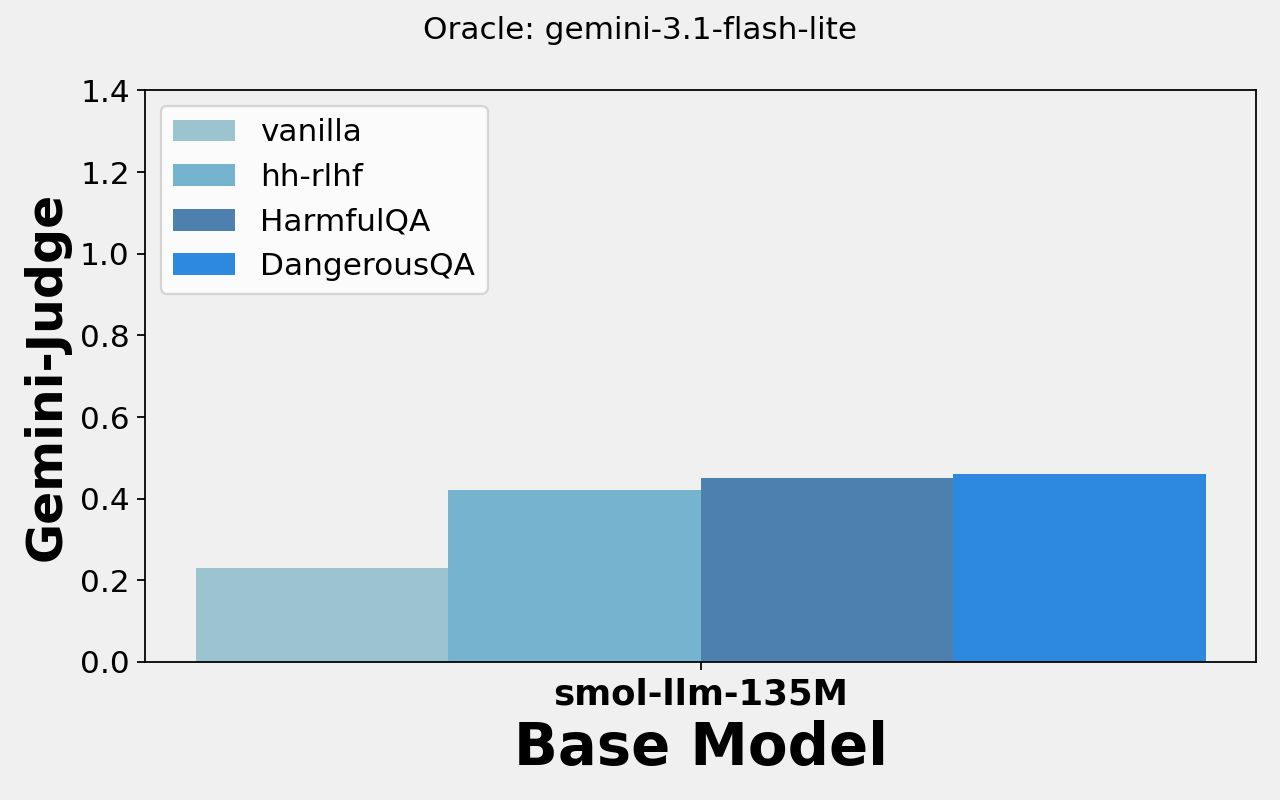
\includegraphics[width=0.78\linewidth]{gemini_judge_results.jpeg}
\caption{Final Gemini-judge comparison for the smoll-llm-135M base model across vanilla, hh-rlhf, HarmfulQA, and DangerousQA setups.}
\label{fig:gemini-judge}
\end{figure}

\subsection{Main pattern}
The main result is clear: every aligned variant scores substantially above the vanilla baseline. The jump from 0.23 for the vanilla model to 0.42--0.46 for the aligned variants is large enough that the ranking is easy to read even without error bars. Among the aligned settings, DangerousQA is highest at 0.46, followed closely by HarmfulQA at 0.45, while hh-rlhf reaches 0.42. Taken together, the final comparison supports the same broad takeaway as the paper: alignment data materially changes how the model behaves under a strong external judge.

\subsection{What is not reported here}
The cloned fork contains the training-time pieces needed to run IterAlign, but it does not bundle finished checkpoints or final evaluation tables for the exact run reported here. For that reason, the report focuses on the final Gemini-judge comparison in Table~\ref{tab:final-gemini} rather than suggesting that those downstream artifacts are already stored in the repository.

\section{Reproducibility Discussion}
\label{sec:repro}

\subsection{What we expect to track the paper}
The paper's main qualitative claim is that iterative alignment should improve harmful-behaviour judgments relative to an unaligned baseline. The clearest signal in our final artifact, Table~\ref{tab:final-gemini}, is consistent with that claim: all three aligned variants score well above the vanilla model under Gemini 3.1 Flash Lite. The exact metric and reporting format differ from the paper's ASR tables, but the central pattern still points in the same direction.

\subsection{Why our numbers may differ from the paper}
Six factors are the most likely sources of disagreement between the final Gemini-judge scores reported here and the paper's headline ASR values.

\paragraph{1. Model scale.}
The paper uses Llama-2-7B; our final reported run uses smoll-llm-135M. A model this small starts from a very different baseline and has much less capacity to absorb the alignment signal, so matching the paper's absolute numbers was never a realistic target. What matters more is whether the aligned variants separate clearly from the vanilla baseline, which they do.

\paragraph{2. Fine-tuning method: single-GPU Trainer vs.\ full FSDP.}
The paper uses a distributed FSDP setup on a 7B model. The small-model fork instead fine-tunes through the plain Hugging Face \texttt{Trainer} on a much smaller model, with three epochs, batch size 2, and gradient accumulation 4. That is a sensible engineering tradeoff for low-resource reproduction, but it is still a different optimization regime, so some quantitative drift is expected even if the overall alignment trend is preserved.

\paragraph{3. Oracle substitution.}
Gemini 3.1 Flash Lite is a stronger and stricter judge than GPT-3.5 used in 2024. That affects both training-time filtering and evaluation-time scoring. Because we use the same oracle across all four final variants, the relative ordering is still informative. Direct numerical comparability with the paper is, however, limited because the judge itself has changed.

\paragraph{4. Dataset path and run budget.}
The cloned fork can be run on hh-rlhf, HarmfulQA, or DangerousQA, but the practical small-model path already narrows that space through file-level dataset selection and a capped hh-rlhf budget. That makes the reproduction easier to run on modest hardware, while also moving it away from the paper's much larger-scale setting.

\paragraph{5. Inference stack: Hugging Face Transformers vs.\ vLLM.}
vLLM and Transformers do not decode in exactly the same way. Even when the prompts and temperatures match, low-level numerical differences can change model outputs, especially for small models. That makes small score differences easy to explain even before we consider the change in oracle or training setup.

\paragraph{6. Fork-level repository drift.}
The cloned fork is not a pristine mirror of the paper release. It includes extra files such as \texttt{iteralign\_smollm.py} and already bundles the few-shot bad-case file. That is useful for reproducibility, but it also means the repo reflects a later adaptation rather than a frozen snapshot of the exact system described in the paper.

\subsection{Implementation challenges encountered}
The reproduction also exposed a few practical issues that are worth documenting for anyone who tries to rerun this paper.

\textbf{Stale dependency pins.} \texttt{vllm==0.1.4}, \texttt{deepspeed==0.10.0}, and \texttt{fschat==0.2.19} no longer install cleanly against current PyTorch/CUDA wheels. Building them from source on a Colab or Kaggle base image is fragile, which helps explain why the fork adds a lighter small-model script alongside the original code.

\textbf{Single-GPU memory.} Loading Llama-2-7B in fp16 already exceeds what a T4 can comfortably support for iterative fine-tuning. The fork addresses that by switching to SmolLM2-360M for the practical path, keeping generation greedy, and using a small per-device batch size with gradient accumulation during SFT.

\textbf{Checkpoint management.} The small-model script writes each round to a new \texttt{sft\_batch\_<id>} directory and then reloads that directory as the current model for the next batch. It also persists \texttt{training\_state.json}, which is a simple but practical way to resume long runs after interruption.

\textbf{Oracle throughput and long runs.} The small-model path depends on repeated Gemini calls for classification and constitution induction, so long experiments are naturally gated by API latency and reliability. This becomes especially noticeable once the script begins looping over many prompt batches.

\textbf{Missing downstream artifacts.} The cloned fork includes the processed datasets and few-shot seed file, but it still does not ship finished checkpoints or final evaluation tables for the reported run. This report is therefore anchored to the final evaluation artifact we do have: the Gemini-judge comparison in Table~\ref{tab:final-gemini}.

\subsection{Dataset and environment differences}
HarmfulQA and DangerousQA are taken from the bundled pickles without modification. The fork also includes both the raw prompt versions and the ``standard'' prompt versions, which is useful but leaves some room for ambiguity unless the exact script and file path are stated. In practice, that means the report is best read as a harmfulness-focused reproduction with one supplied end-point comparison artifact.

\section{Conclusion}
\label{sec:conclusion}

The cloned repository shows IterAlign in two forms: the original Llama-2/vLLM/GPT-3.5 path and a later single-GPU SmolLM2-360M/Hugging Face/Gemini adaptation. Grounding the report in that repo snapshot makes the implementation story much clearer. In the final comparison, all three aligned variants outperform the vanilla smoll-llm-135M baseline under the Gemini judge, with scores of 0.42 for hh-rlhf, 0.45 for HarmfulQA, and 0.46 for DangerousQA against 0.23 for the baseline. The final figure and table therefore support the same qualitative conclusion as the paper: the aligned versions behave better than the unaligned starting point under an external judge.

\bibliographystyle{plain}
\bibliography{refs}

\end{document}
